\begin{enumerate}[label=\bfseries Câu \arabic*:]
	
	
	%%%%%%%%%%%%%%CÂU2%%%%%%%%%%
	\item \mkstar{1}
	
	\cauhoi{Một máy biến áp có số vòng dây của cuộn sơ cấp lớn hơn số vòng dây của cuộn thứ cấp. Máy biến áp này có tác dụng
		\begin{mcq}
			\item tăng cường độ dòng điện, giảm điện áp.
			\item giảm cường độ dòng điện, tăng điện áp.
			\item tăng cường độ dòng điện, tăng điện áp.
			\item giảm cường độ dòng điện, giảm điện áp.
		\end{mcq}
}	
		\loigiai{
			\textbf{Đáp án: A.}
			
			Máy biến áp có số vòng cuộn sơ cấp lớn hơn số vòng cuộn thứ cấp là máy hạ áp và có tác dụng làm tăng cường độ dòng điện.
			
			}	
	
	%%%%%%%%%%%%%%CÂU2%%%%%%%%%%
	\item \mkstar{1}
	
	\cauhoi{Hoạt động của máy biến áp dựa trên
		\begin{mcq}(2)
			\item hiên tượng tự cảm.
			\item hiên tượng cảm ứng điện từ.
			\item từ trường quay.
			\item tác dụng của lực từ.
		\end{mcq}
}	
		\loigiai{
			\textbf{Đáp án: B.}
			
			Hoạt động của máy biến áp dựa trên hiên tượng cảm ứng điện từ.
			
			}
	
	%%%%%%%%%%%%%%CÂU3%%%%%%%%%%
	\item \mkstar{1}
	
	\cauhoi{Nguyên nhân chủ yếu gây ra sự hao phí năng lượng trong máy biến thế là do
		\begin{mcq}
			\item hao phí năng lượng dưới dạng nhiệt năng tỏa ra ở các cuộn sơ cấp và thứ cấp của máy biến thế.
			\item lõi sắt có từ trở và gây dòng Fu-cô.
			\item có sự thất thoát năng lượng dưới dạng bức xạ điện từ.
			\item Cả 3 ý kiến trên.
		\end{mcq}
}	
		\loigiai{
			\textbf{Đáp án: D.}
			
			Nguyên nhân chủ yếu gây ra sự hao phí năng lượng trong máy biến thế là do
			\begin{itemize}
				\item hao phí năng lượng dưới dạng nhiệt năng tỏa ra ở các cuộn sơ cấp và thứ cấp của máy biến thế.
				\item lõi sắt có từ trở và gây dòng Fu-cô.
				\item có sự thất thoát năng lượng dưới dạng bức xạ điện từ.
			\end{itemize}
			
			}
	
	%%%%%%%%%%%%%%CÂU4%%%%%%%%%%
	\item \mkstar{1}
	
	\cauhoi{Vai trò của máy biến thế trong truyền tải điện năng là
		\begin{mcq}
			\item giảm điện trở của dây dẫn trên đường truyền tải để giảm hao phí trên đường truyền tải.
			\item tăng hiệu điện thế truyền tải để giảm hao phí trên đường truyền tải.
			\item giảm hiệu điện thế truyền tải để giảm hao phí trên đường truyền tải.
			\item giảm sự thất thoát năng lượng dưới dạng bức xạ sóng điện từ.
		\end{mcq}
}	
		\loigiai{
			\textbf{Đáp án: B.}
			
			Vai trò của máy biến thế trong truyền tải điện năng là tăng hiệu điện thế truyền tải để giảm hao phí trên đường truyền tải.
			
			}	
	
	%%%%%%%%%%%%%%CÂU5%%%%%%%%%%
	\item \mkstar{2}
	
	\cauhoi{Chọn câu đúng.
		\begin{mcq}
			\item Khi mạch thứ cấp hở dòng điện ở cuộn sơ cấp luôn bằng 0. 
			\item Dòng điện trong cuộn sơ cấp là dòng điện cảm ứng.
			\item Cuộn sơ cấp là máy thu điện.
			\item Cường độ dòng điện trong mạch sơ cấp khác nhau trong hai trường hợp mạch thứ cấp kín và hở.
		\end{mcq}
}	
		\loigiai{
			\textbf{Đáp án: D.}
			
		Cường độ dòng điện trong mạch sơ cấp khác nhau trong hai trường hợp mạch thứ cấp kín và hở.	
			
			}	
	
	%%%%%%%%%%%%%%CÂU6%%%%%%%%%%
	\item \mkstar{2}
	
	\cauhoi{Máy biến thế có thể dùng để biến đổi hiệu điện thế của nguồn điện nào sau đây?
		\begin{mcq}(2)
			\item Pin.
			\item Ac-quy.
			\item Nguồn điện xoay chiều AC.
			\item Nguồn điện một chiều DC.
		\end{mcq}
}	
		\loigiai{
			\textbf{Đáp án: C.}
			
			Máy biến thế có thể dùng để biến đổi hiệu điện thế của nguồn điện xoay chiều AC.
			
			}	
	
	%%%%%%%%%%%%%%CÂU7%%%%%%%%%%
	\item \mkstar{2}
	
	\cauhoi{Người ta dùng lõi thép kĩ thuật điện trong máy biến áp, mục đích chính là để
		\begin{mcq}
			\item làm mạch dẫn dòng điện từ cuộn sơ cấp sang cuộn thứ cấp.
			\item làm mạch từ và tăng cường từ thông qua các cuộn dây.
			\item làm giảm hao phí do tỏa nhiệt bởi dòng điện Fu-cô.
			\item làm khung lắp cuộn sơ cấp và cuộn thứ cấp trên nó.
		\end{mcq}
	}
		\loigiai{
			\textbf{Đáp án: B.}
			
			Người ta dùng lõi thép kĩ thuật điện trong máy biến áp, mục đích chính là để làm mạch từ và tăng cường từ thông qua các cuộn dây.
			
			}
	
	%%%%%%%%%%%%%%CÂU8%%%%%%%%%%
	\item \mkstar{2}
	
	\cauhoi{Biện pháp nào sau đây \textbf{không} góp phần tăng hiệu suất của máy biến áp?
		\begin{mcq}
			\item Đặt các lá sắt của lõi sắt song song với mặt phẳng chứa các đường sức từ.
			\item Dùng lõi sắt gồm nhiều lá sắt mỏng ghép cách điện với nhau.
			\item Dùng dây có điện trở suất nhỏ là dây quấn biến áp.
			\item Dùng lõi sắt có điện trở suất nhỏ.
		\end{mcq}
}	
		\loigiai{
			\textbf{Đáp án: D.}
			
			Dùng lõi sắt có điện trở suất nhỏ thì điện trở nhỏ, giảm công suất nên không góp phần tăng hiệu suất của máy biến áp.
			
			}	
	
	%%%%%%%%%%%%%%CÂU9%%%%%%%%%%
	\item \mkstar{2}
	
	\cauhoi{Người ta cần truyền một công suất điện 200 kW từ nguồn điện có điện áp 5000 V trên đường dây có điện trở tổng cộng $20\ \Omega$ và hệ số công suất bằng 1. Độ giảm thế trên đường dây tải điện là
		\begin{mcq}(4)
			\item 40 V.
			\item 400 V.
			\item 80 V.
			\item 800 V.
		\end{mcq}
}	
		\loigiai{
			\textbf{Đáp án: D.}
			
			\begin{itemize}
				\item Áp dụng công thức công suất hao phí do tỏa nhiệt trên đường dây
				
				\begin{equation*}
					\Delta P = I^2R =R\dfrac{P^2}{(U \cos \varphi)^2}.
				\end{equation*}
				\item Suy ra độ giảm thế trên đường dây truyền tải
				\begin{equation*}
					\Delta U = IR = \dfrac{P}{U \cos \varphi}R = 800\ \text{V}.
				\end{equation*}
			\end{itemize}
			
			}
	
	%%%%%%%%%%%%%%CÂU10%%%%%%%%%%
	\item \mkstar{2}
	
	\cauhoi{Một máy tăng áp có tỉ số vòng dây giữa hai cuộn dây là 2. Đặt vào hai đầu cuộn sơ cấp một điện áp xoay chiều có tần số $\SI{50}{Hz}$. Tần số dòng điện hai đầu cuộn thứ cấp bằng
		\begin{mcq}(4)
			\item $\SI{50}{Hz}$.
			\item $\SI{25}{Hz}$.
			\item $\SI{100}{Hz}$.
			\item $50\sqrt{2}\ \SI{}{Hz}$.
		\end{mcq}
	}
		\loigiai{
			\textbf{Đáp án: A.}
			
			Máy biến áp không làm thay đổi tần số của dòng điện qua nó.
			
			}
	
	%%%%%%%%%%%%%%CÂU11%%%%%%%%%%
	\item \mkstar{2}
	
	\cauhoi{Trạm phát điện truyền đi công suất $\SI{550}{kW}$, điện áp nơi phát bằng $\SI{10}{kV}$. Muốn độ giảm điện áp trên dây tải không vượt quá $10\%$ điện áp nơi phát thì điện trở của dây tải điện không được vượt quá giá trị
		\begin{mcq}(4)
			\item $\SI{18}{\ohm}$.
			\item $\SI{11}{\ohm}$.
			\item $\SI{55}{\ohm}$.
			\item $\SI{5,5}{\ohm}$.
		\end{mcq}
}	
		\loigiai{
			\textbf{Đáp án: A.}
			
			Công suất hao phí là
			$$\Delta=R\left(\dfrac{P}{U}\right)^2\leq \dfrac{10}{100}P\Rightarrow R\leq \dfrac{0,1U^2}{P}=\SI{18}{\ohm}.$$
			
			}
	
	%%%%%%%%%%%%%%CÂU12%%%%%%%%%%
	\item \mkstar{2}
	
	\cauhoi{Một máy biến áp lý tưởng có tỉ số giữa số vòng dây của cuộn sơ cấp và số vòng dây của cuộn thứ cấp bằng 10. Mắc một bóng đèn sợi đốt loại $\SI{24}{V}$ – $\SI{24}{W}$ vào hai đầu cuộn thứ cấp thì đèn sáng bình thường. Cường độ dòng điện hiệu dụng trong cuộn sơ cấp bằng
		\begin{mcq}(4)
			\item $\SI{0,2}{A}$.
			\item $\SI{0,5}{A}$.
			\item $\SI{0,1}{A}$.
			\item $\SI{2}{A}$.
		\end{mcq}
}	
		\loigiai{
			\textbf{Đáp án: C.}
			
			Dòng điện qua đèn để đèn sáng bình thường
			$$I_\textrm{đ}=I_2=\dfrac{P}{U}=\SI{1}{A}.$$
			
			Dòng điện ở cuộn sơ cấp là
			$$I_1=\dfrac{I_2}{n}=\SI{0,1}{A}.$$
			}
	
	%%%%%%%%%%%%%%CÂU13%%%%%%%%%%
	\item \mkstar{2}
	
	\cauhoi{Đặt vào hai đầu cuộn sơ cấp của một máy biến áp lí tưởng (bỏ qua hao phí) một điện áp xoay chiều có giá trị hiệu dụng không đổi thì điện áp hiệu dụng giữa hai đầu cuộn thứ cấp để hở là $100\ V$. Ở cuộn thứ cấp, nếu giảm bớt n vòng dây thì điện áp hiệu dụng giữa hai đầu để hở của nó là $U$, nếu tăng thêm $n$ vòng dây thì điện áp đó là $2U$. Nếu tăng thêm $3n$ vòng dây ở cuộn thứ cấp thì điện áp hiệu dụng giữa hai đầu để hở của cuộn này bằng
		\begin{mcq}(4)
			\item $\SI{200}{V}$.
			\item $\SI{220}{V}$.
			\item $\SI{110}{V}$.
			\item $\SI{100}{V}$.
		\end{mcq}
}	
		\loigiai{
			\textbf{Đáp án: A.}
			
			Ta có: $$\left\{\begin{array}{l}\dfrac{\mathrm{N}_{2}}{\mathrm{N}_{1}}=\dfrac{100}{\mathrm{U}_{1}} \\ \dfrac{\mathrm{N}_{2}-\mathrm{n}}{\mathrm{N}_{1}}=\dfrac{\mathrm{U}}{\mathrm{U}_{1}} \Rightarrow \mathrm{N}_{2}=3 \mathrm{n} \\ \dfrac{\mathrm{N}_{2}+\mathrm{n}}{\mathrm{N}_{1}}=\dfrac{2 \mathrm{U}}{\mathrm{U}_{1}}.\end{array}\right.$$
			
			Vậy khi số vòng tăng 3n vòng thì tỉ số $$\dfrac{N_2+3n}{N_1}=\dfrac{2N_2}{N_1}=\dfrac{U_2}{U_1}\Rightarrow\dfrac{200}{U_1}=\dfrac{U_2}{U_1}\Rightarrow \SI{200}{V}.$$
			
			}
	
	%%%%%%%%%%%%%%CÂU14%%%%%%%%%%
	\item \mkstar{2}
	
	\cauhoi{Cho một máy biến áp có hiệu suất $80\%$. Cuộn sơ cấp có 100 vòng, cuộn thứ cấp có 200 vòng. Mạch sơ cấp lý tưởng, đặt vào hai đầu cuộn sơ cấp điện áp xoay chiều có giá trị hiệu dụng 100 V và tần số 50 Hz. Hai đầu cuộn thứ cấp nối với một cuộn dây có điện trở $50\ \Omega$, độ tự cảm $\dfrac{\text{0,5}}{\pi}\ \text{H}$. Cường độ dòng điện hiệu dụng mạch sơ cấp nhận giá trị
		\begin{mcq}(4)
			\item 5 A.
			\item 10 A.
			\item 2 A.
			\item 2,5 A.
		\end{mcq}
}	
		\loigiai{
			\textbf{Đáp án: A.}
			
			\begin{itemize}
				\item Áp dụng công thức suy ra điện áp của cuộn thứ cấp
				\begin{equation*}
					\dfrac{U_2}{U_1}=\dfrac{N_2}{N_1} \Rightarrow U_2= \dfrac{N_2}{N_1}U_1 = 200\ \text{V}.
				\end{equation*}
				\item Cường độ dòng điện qua cuộn thứ cấp
				\begin{equation*}
					I_2 = \dfrac{U_2}{\sqrt{R^2+Z_L^2}}= 2\sqrt 2\ \text{A}.
				\end{equation*}
				\item Hiệu suất của máy biến áp 
				\begin{equation*}
					H=\dfrac{I^2_2R}{U_1I_1}.
				\end{equation*}
				\item Suy ra cường độ dòng điện qua cuộn sơ cấp 
				\begin{equation*}
					I_1= \dfrac{I^2_2R}{HU_1}=5\ \text{A}.
				\end{equation*}
			\end{itemize}
			
			}
	
	%%%%%%%%%%%%%%CÂU15%%%%%%%%%%
	\item \mkstar{3}
	
	\cauhoi{Một đường dây có điện trở tổng cộng $4\ \Omega$ dẫn một dòng điện xoay chiều một pha từ nơi sản xuất đến nơi tiêu dùng. Điện áp hiêu dụng ở nguồn điện lúc phát ra là 10 kV, công suất điện là 400 kW. Hệ số công suất của mạch điện là $\cos \varphi = \text {0,8}$. Có bao nhiêu phần trăm công suất bị hao phí trên đường dây do tỏa nhiệt?
		
		\begin{mcq}(4)
			\item 1,6$\%$.        
			\item 2,5$\%$.
			\item 6,4$\%$.       
			\item 10$\%$.
		\end{mcq}
}	
		\loigiai{
			\textbf{Đáp án: B.}
			
			\begin{itemize}
				\item  Công suất hao phí trên đường dây tải điện
				\begin{equation*}
					\Delta P= I^2R = \left(\dfrac{P}{U\cos \varphi}\right)^2R.
				\end{equation*}
				\item Hiệu suất truyền tải điện 
				\begin{equation*}
					H = \dfrac{P-\Delta P}{P}=1-\dfrac{\Delta P}{P}.
				\end{equation*}
				\item Phần trăm công suất bị hao phí
				\begin{equation*}
					h= \dfrac{\Delta P}{P}= \dfrac{PR}{U^2 \cos^2 \varphi} = \text{0,025}= \text{2,5}\ \%.
				\end{equation*}
			\end{itemize}
			
			
			}
	
	%%%%%%%%%%%%%%CÂU16%%%%%%%%%%
	\item \mkstar{3}
	
	\cauhoi{Ở trạm phát điện xoay chiều một pha có điện áp hiệu dụng 110 kV, truyền đi công suất điện 1000 kW trên đường dây dẫn có điện trở $20\ \Omega$. Hệ số công suất của đoạn mạch $\cos \varphi =\text{0,9}$. Điện năng hao phí trên đường dây trong 30 ngày là
		
		\begin{mcq}(4)
			\item 5289 kWh.
			\item 61,2 kWh.
			\item 145,5 kWh.
			\item 1469 kWh.
		\end{mcq}
	}
		\loigiai{
			\textbf{Đáp án: D.}
			
			\begin{itemize}
				\item Công suất hao phí trên đường dây tải điện
				\begin{equation*}
					\Delta P = \left(\dfrac{P}{U\cos \varphi}\right)^2 \cdot R = \text{2040,6}\ \text{W}.
				\end{equation*}
				\item Thời gian 30 ngày $t=30 \cdot 24 =720 \ \text{giờ}$.
				\item Điện năng hao phí trên đường dây trong 30 ngày
				\begin{equation*}
					A= \Delta P \cdot t = 1469232\ \text{W} \approx  1469\ \text{kWh}.
				\end{equation*}
			\end{itemize}
			
			}
	
	%%%%%%%%%%%%%%CÂU17%%%%%%%%%%
	\item \mkstar{3}
	
	\cauhoi{Người ta truyền tải điện xoay chiều một pha từ một trạm phát điện đến nơi tiêu thụ bằng dây dẫn có tổng chiều dài 20 km. Dây dẫn làm bằng kim loại có điện trở suất $\text{2,5}\cdot 10^{-8}\ \Omega m$, tiết diện $\text{0,4}\ \text{cm}^2$, hệ số công suất của mạch điện là 1. Điện áp hiệu dụng và công suất truyền đi ở trạm phát điện là $10\ \text{kV}$ và 500 kW. Hiệu suất truyền tải điện là
			\begin{mcq}(4)
				\item 93,75$\%$.        
				\item 96,14$\%$.
				\item 97,41$\%$.        
				\item 96,88$\%$.
			\end{mcq}
	}	
			\loigiai{
				\textbf{Đáp án: A.}
				
				\begin{itemize}
					\item Điện trở đường dây tải điện
					\begin{equation*}
						R = \rho \dfrac{l}{S}=\text{12,5}\ \Omega.
					\end{equation*}
					\item  Công suất hao phí trên đường dây tải điện
					\begin{equation*}
						\Delta P= I^2R = \left(\dfrac{P}{U\cos \varphi}\right)^2R= \text{31250}\ \text{W}.
					\end{equation*}
					\item Hiệu suất truyền tải điện 
					\begin{equation*}
						H = \dfrac{P-\Delta P}{P}=1-\dfrac{\Delta P}{P}= \text{93,75}\% .
					\end{equation*}
				\end{itemize}
				
				}
		
		%%%%%%%%%%%%%%CÂU18%%%%%%%%%%
		\item \mkstar{3}
		
		\cauhoi{Một máy phát điện xoay chiều có công suất 1000 kW. Dòng điện nó phát ra sau khi tăng thế được truyền đi xa bằng một dây dẫn có tổng chiều dài 200 km có đường kính 0,39 cm và bằng hợp kim có điện trở suất bằng $\text {1,8} \cdot 10^{-8}\ \Omega \text{m}$. Biết hệ số công suất đường dây bằng 1. Tính công suất hao phí trên đường dây nếu điện áp đưa lên là 50 kV.
			\begin{mcq}(4)
				\item 0,16 MW.
				\item 0,03 MW.
				\item 0,2 MW.
				\item 0,12 MW.
			\end{mcq}
	}	
			\loigiai{
				\textbf{Đáp án: A.}
				
				\begin{itemize}
					\item Diện tích hình tròn
					\begin{equation*}
						S=\pi r^2=\pi \dfrac{d^2}{4}=\text{1,19}\cdot 10^{-5}\ \text{cm}^2.
					\end{equation*}
					\item Điện trở đường dây
					\begin{equation*}
						R=\rho \dfrac{l}{S}= 301\ \Omega.
					\end{equation*}
					\item Công suất hao phí trên đường dây
					\begin{equation*}
						\Delta P =R\dfrac{P^2}{(U \cos \varphi)^2} \approx \text {0,12} \cdot 10^{6}\ \text{W}
					\end{equation*}
				\end{itemize}	
				
				}
		
		%%%%%%%%%%%%%%CÂU19%%%%%%%%%%
		
			\item \mkstar{3}
			
			\cauhoi{Điện năng được truyền tải từ nhà máy thủy điện đến khu dân cư có công suất tiêu thụ không đổi. Khi truyền đi với điện áp là $U$  thì độ giảm điện áp trên đường dây tải điện bằng $\dfrac{U}{10}$. Coi cường độ dòng điện trong mạch luôn cùng pha với điện áp đặt lên đường dây, điện trở của đường dây luôn không đổi. Để hao phí trên đường dây giảm 144 lần thì cần tăng điện áp truyền đi lên gần nhất giá trị nào sau đây?
				\begin{mcq}(4)
					\item 8 lần.
					\item 9 lần.
					\item 10 lần.
					\item 11 lần.
				\end{mcq}
	}		
				\loigiai{
				\textbf{Đáp án: D.}
					
					$P_\text{tt} =U_\text{tt} I$ không đổi nên $I$ và $U_\text{tt}$ tỉ lệ nghịch với nhau.
					
					$\Delta P = I^2R$ suy ra $\Delta P $ giảm 144 lần thì $I$ giảm 12 lần (lưu ý, ta không dùng $\Delta P =\dfrac{PR}{U^2}$ để biện luận vì bài toán không ràng buộc điều kiện $P$  không đổi)		
					Ta lập bảng số liệu cho hai trường hợp:
					
					\begin{center}
						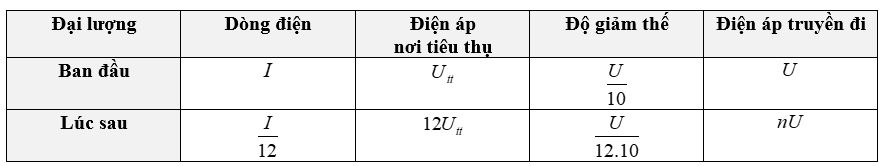
\includegraphics[scale=0.8]{../figs/VN12-PH-21-P-015-1-1.jpg}
					\end{center}
					
					Ta có: 
					
					$12U_\text{tt} =nU - \dfrac{U}{12 \cdot 10} \Rightarrow 12 \left(U-\dfrac{U}{10}\right) = nU -	\dfrac{U}{12 \cdot 10} \Rightarrow n = \text{10,8}$.
					
					}
			
			%%%%%%%%%%%%%%CÂU2%%%%%%%%%%
			\item \mkstar{3}
			
			\cauhoi{Điện năng được truyền từ nơi phát đến một khu dân cư bằng đường dây một pha với hiệu suất truyền tải là $80\%$. Coi hao phí điện năng chỉ do tỏa nhiệt trên đường dây và không vượt quá $20\%$. Nếu công suất sử dụng điện của khu dân cư này tăng $50\%$ và giữ nguyên điện áp ở nơi phát thì hiệu suất truyền tải điện năng trên chính đường dây đó gần nhất giá trị nào sao đây?
				\begin{mcq}(4)
					\item $80\%$.
					\item $70\%$.
					\item $90\%$.
					\item $85\%$.
				\end{mcq}
		}	
				\loigiai{
					\textbf{Đáp án: B.}
					
					Nhận thấy rằng, trong trường hợp thứ hai của bài toán truyền tải, công suất nơi tiêu thụ tăng. Do đó công suất truyền tải lúc sau cũng phải tăng theo.
					
					Vì điện áp ở nơi truyền tải được giữ không đổi, nếu tăng $nP$  thì dòng điện lúc sau là $nI$. Ta lập bảng tỉ lệ
					\begin{center}
						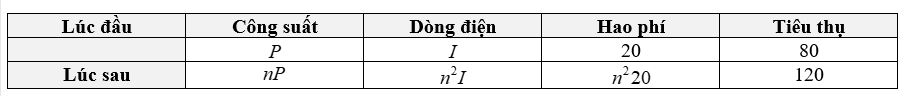
\includegraphics[scale=0.8]{../figs/VN12-PH-21-P-015-1-2.jpg}
					\end{center}
					Ta có 
					
					$100n =20n^2 + 120$ suy ra $n =3$ hoặc $n=2$.
					
					$n=2$ thì $\dfrac{\Delta P}{P} = \dfrac{20n}{100} = \text{0,4} \Rightarrow H = \text{0,6}\ \text{nhận}$.
					
					$n=3$ thì $\dfrac{\Delta P}{P} = \dfrac{20n}{100} = \text{0,6} > \text{0,5} \Rightarrow H = \text{0,4}\ \text{loại}$.
					
					}
			
			%%%%%%%%%%%%%%CÂU3%%%%%%%%%%
			\item \mkstar{3}
			
			\cauhoi{Điện năng được truyền từ trạm phát điện đến nơi tiêu thụ bằng đường dây tải điện một pha. Ban đầu hiệu suất truyền tải là $60\%$. Cho công suất truyền đi không đổi và hệ số công suất ở nơi tiêu thụ (cuối đường dây tải điện) luôn bằng 0,8. Để giảm hao phí trên đường dây 4 lần thì cần phải tăng điện áp hiệu dụng ở trạm phát điện lên $n$  lần. Giá trị của $n$  là
				\begin{mcq}(4)
					\item 2,0.
					\item 2,1.
					\item 2,3.
					\item 2,2.
				\end{mcq}
		}	
				\loigiai{
					\textbf{Đáp án: D.}
					
					Ta biễu diễn mối liên hệ giữa các điện áp trong quá trình truyền tải
					\begin{center}
						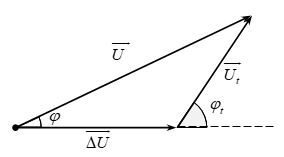
\includegraphics[scale=0.8]{../figs/VN12-PH-21-P-015-1-3.jpg}
					\end{center}
					$$U \cos \varphi =U_\text{t} \cos \varphi_\text{t}$$.
					$$P_\text{tt} = HP \Rightarrow U_\text{t} I \cos \varphi_\text{t} = H(UI \cos \varphi) \Rightarrow U\cos \varphi = \dfrac{U_\text{t} \cos \varphi_\text{t}}{H}$$
					
					Từ hai phương trình trên, ta có $\tan \varphi = H \tan \varphi_\text{t}$. 
					
					Tiến hành lập bảng tỉ lệ
					\begin{center}
						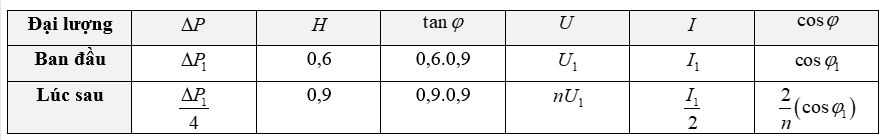
\includegraphics[scale=0.8]{../figs/VN12-PH-21-P-015-1-4.jpg}
					\end{center}
					Ta có
					
					$$\left (\dfrac{\cos \varphi_2}{\cos \varphi_1}\right)^2 = \dfrac{4}{n^2} = \dfrac {1+\tan ^2 \varphi_1}{1+ \tan^2 \varphi_2} \Rightarrow n \approx \text{2,2}$$
					
					}
			
			%%%%%%%%%%%%%%CÂU4%%%%%%%%%%
			\item \mkstar{2}
			
			\cauhoi{Một trạm phát điện truyền đi công suất 1000 kW bằng dây dẫn có điện trở tổng cộng $8\ \Omega$  điện áp ở hai cực của máy là 1000 V. Hai cực của máy được nối với hai đầu cuộn sơ cấp của máy tăng áp lý tưởng mà số vòng dây của cuộn thứ cấp gấp 10 lần số vòng dây cuộn sơ cấp. Biết hệ số công suất của đường dây bằng 1. Hiệu suất quá trình truyền tải:
				\begin{mcq}(4)
					\item $92\%$..
					\item $95\%$..
					\item $80\%$..
					\item $87\%$..
				\end{mcq}
		}	
				\loigiai{
					\textbf{Đáp án: A.}
					
					Điện áp phát ra ở hai đầu cuộn thứ cấp: 
					
					$$\dfrac{U_1}{U_2} =\dfrac{N_1}{N_2} \Rightarrow U_2 =U_1 \dfrac{N_2}{N_1} = 10^4\ \text{V}$$
					
					Công suất hao phí: $$\Delta P = \dfrac{P^2R}{U^2_2 \cos^2 \varphi}$$
					
					Hiệu suất quá trình truyền tải: $$H = 1- \dfrac{\Delta P}{P} = \text{0,92} = 92\%$$
					
				}
			
			%%%%%%%%%%%%%%CÂU5%%%%%%%%%%
			\item \mkstar{3}
			
			\cauhoi{Khi đặt một điện áp xoay chiều có giá trị hiệu dụng không đổi vào hai đầu cuộn sơ cấp của một máy biến áp thì điện áp hiệu dụng ở hai đầu thứ cấp để hở là 20 V. Khi tăng số vòng dây cuộn thứ cấp thêm 60 vòng thì điện áp hiệu dụng hai đầu thứ cấp là 25 V. Khi giảm số vòng dây thứ cấp đi 90 vòng thì điện áp hiệu dụng hai đầu thứ cấp để hở là
				\begin{mcq}(4)
					\item 17,5 V.
					\item 15 V.
					\item 10 V.
					\item 12,5 V.
				\end{mcq}
		}	
				\loigiai{
					\textbf{Đáp án: D.}
					
					Ta có:$$\dfrac{U_1}{20} =\dfrac{N_1}{N_2} (1); \dfrac{U_1}{25} = \dfrac{N_1}{N_2+60} (2); \dfrac{U_1}{U_3} = \dfrac{N_1}{N_2 - 90} (3)$$
					Chia vế với vế của (1) cho (2), được: $$\dfrac{25}{20} = \dfrac{N_2 +60}{N_2} \Rightarrow N_2 = 240\ \text{vòng}$$
					Chia vế với vế của (1) cho (3), được: $$\dfrac{U_3}{20}=\dfrac{N_2 - 90}{N_2} \Rightarrow U_3 =\text{12,5}\ \text{V}$$
					
					}
			
			%%%%%%%%%%%%%%CÂU6%%%%%%%%%%
			\item \mkstar{3}
			
			\cauhoi{Điện năng từ một trạm phát điện được đưa đến một khu tái định cư bằng dây truyền tải một pha. Cho biết, nếu điện áp tạo đầu truyền đi tăng từ $U$ lên $2U$ thì số hộ dân được trạm cung cấp đủ điện năng từ 120 lên 144. Cho rằng chỉ tính đến hao phí trên đường dây, công suất tiêu thụ điện của các hộ dân đều như nhau, công suất của trạm phát không đổi và hệ số công suất trong các trường hợp đều bằng nhau. Nếu điện áp truyền đi là $4U$ thì trạm phát này cung cấp đầy đủ điện năng cho
				\begin{mcq}(4)
					\item 168 hộ dân.
					\item 504 hộ dân.
					\item 192 hộ dân.
					\item 150 hộ dân.
				\end{mcq}
	}		
				\loigiai{
				\textbf{Đáp án: D.}
					
					Ta xét các trường hợp:
					
					+ Khi $U$ tăng lên 2 $\Rightarrow$ công suất hao phí giảm 4: $\dfrac{\Delta P}{4}$.  
					
					$\Rightarrow$ Công suất điện cấp cho hộ dân tăng lên $\dfrac{3\Delta P}{4}$  tương ứng với $144-120 =24$ hộ dân.
					
					+ Khi $U$ tăng lên 4 $\Rightarrow$ công suất hao phí giảm 16: $\dfrac{\Delta P}{16}$.
					
					$\Rightarrow$ Công suất điện cấp cho hộ dân tăng lên $\dfrac{15\Delta P}{16}$  tương ứng với $\dfrac{\dfrac{15 \Delta P}{16} \cdot 24}{\dfrac{3\Delta P}{4}}=30$ hộ dân.
					
					$\Rightarrow$ Điện áp $4U$ sẽ cấp đủ cho $120 + 30 =150$ hộ dân. 
					
					}
			
			%%%%%%%%%%%%%%CÂU7%%%%%%%%%%
			\item \mkstar{3}
			
			\cauhoi{Điện năng được truyền từ một nhà máy phát điện có công suất không đổi đến một khu công nghiệp bằng đường dây tải điện một pha. Nếu điện áp hiệu dụng truyền đi là $U$ và ở khu công nghiệp lắp một máy hạ áp lý tưởng có hệ số biến áp là 54 thì đáp ứng được $\dfrac{12}{13}$ nhu cầu sử dụng điện của công nghiệp. Coi cường độ dòng điện và điện áp luôn cùng pha. Muốn cung cấp đủ điện năng cho khu công nghiệp với điện áp truyền đi là $2U$ thì ở khu công nghiệp cần dùng máy hạ áp lý tưởng hệ số biến áp là
				\begin{mcq}(4)
					\item 114.
					\item 111.
					\item 117.
					\item 108.
				\end{mcq}
		}	
				\loigiai{
					\textbf{Đáp án: C.}
					
					+ Gọi $U_0$ là điện áo cuộn thứ cấp. Khi $k=54$ suy ra điện áp cuộn sơ cấp là $54U_0$.
					
					Khi $k=n$ thì điện áp cuộn sơ cấp là $nU_0$.
					
					+ Khi điện áp hiệu dụng là $U$ thì hao phí là $\Delta P \Rightarrow P - \Delta P =12 (1)$.
					+ Khi điện áp hiệu dụng là $2U$ thì hao phí là $\dfrac{\Delta P}{4} \Rightarrow P- \dfrac{\Delta P}{4} =13(2)$.
					
					+ Giải (1) và (2) ta được: $P =\dfrac{40}{3}\ \text{W}$ và $\Delta P =\dfrac{4}{3}$.
					
					Suy ra:
					
					$$H_1 =\dfrac{P-\Delta P}{P} =\text{0,9} = \dfrac{54U_0}{U} \Rightarrow \dfrac{U_0}{U} = \dfrac{1}{60}$$
					$$H_2 = \dfrac{P-\dfrac{\Delta P}{4}}{P} = \dfrac{39}{40} =\dfrac{nU_0}{2U} \Rightarrow n = 117$$	
					
					
					}
			
			%%%%%%%%%%%%%%CÂU8%%%%%%%%%%
			\item \mkstar{3}
			
		\cauhoi{Một máy hạ thế có tỉ số giữa số vòng dây cuộn sơ cấp và số vòng cuộn thứ cấp là $k$ $(k>1)$. Nhưng do không ghi kí hiệu trên máy nên không biết được số vòng trên các cuộn sơ cấp và thứ cấp. Một người đã dùng máy biến thế trên lần lượt đấu hai đầu mỗi cuộn dây của máy vào mạng điện xoay chiều có điện áp hiệu dụng không đổi $U$ và dùng vôn kế đo điện áp hiệu dụng ở hai đầu cuộn dây còn lại. Kết quả lần đo thứ nhất thu được là 250 V, lần đo thứ 2 là 10 V. Tỉ số $k$ bằng
				\begin{mcq}(4)
					\item 8.
					\item 2.
					\item 5.
					\item 16.
				\end{mcq}
		}	
				\loigiai{
					\textbf{Đáp án: D.}
					
					Do đây là máy hạ thế nên số vòng cuộn sơ cấp $N_1$  nhiều hơn số vòng cuộn thứ cấp $N_2$
					
					Lần đo thứ nhất: $$k = \dfrac{N_1}{N_2} = \dfrac{250}{U} (1)$$
					
					Lần đo thứ hai: $$k =\dfrac{N_1}{N_2} =\dfrac{U}{10} (2)$$
					
					Từ (1) và (2) ta có $$\dfrac{250}{U} =\dfrac{U}{10} \Rightarrow U =50\ \text{V} \Rightarrow k =5$$
					
					}
			
			%%%%%%%%%%%%%%CÂU9%%%%%%%%%%
			\item \mkstar{3}
			
			\cauhoi{Cho một máy biến áp lí tưởng, cuộn sơ cấp có $N_1$ vòng dầy, cuộn thứ cấp có $N_2$ vòng dây. Nếu giữ nguyên điện áp hiệu dụng hai đầu cuộn sơ cấp, rồi quấn thêm vào cuộn sơ cấp 25 vòng thì điện áp hiệu dụng ở hai đầu cuộn thứ cấp giảm đi $\dfrac{100}{13}\%$ . Còn nếu quấn thêm vào cuộn thứ cấp 25 vòng và muốn điện áp hiệu dụng hai đầu cuộn này không đổi thì phải giảm điện áp hiệu dụng hai đầu cuộn sơ cấp $\dfrac{100}{13}\%$ . Hệ số máy biến áp $k =\dfrac{N_1}{N_2}$  là
				\begin{mcq}(4)
					\item 6,5.
					\item 13.
					\item 6.
					\item 12.
				\end{mcq}
		}	
				\loigiai{
					\textbf{Đáp án: C.}
					
					Hệ số máy biến áp: $k= \dfrac{N_1}{N_2} =\dfrac{U_1}{U_2}$.
					
					+	Lần đo thứ nhất:
					
					Hiệu điện thế và số vòng dây trên cuộn sơ cấp: $U_1; N_1 + 25$.
					
					Hiệu điện thế và số vòng dây trên cuộn thứ cấp: $U'_2 =U_2 -\dfrac{1}{13}U_2; N_2$.
					
					Ta có: $$\dfrac{N_1 +25}{N_2} =\dfrac{U_1}{U_2 \left(1-\dfrac{1}{13}\right)} \Leftrightarrow k+\dfrac{25}{N_2} = \dfrac{13}{12} k$$
					
					$$N_2 =\dfrac{300}{k}; N_1 =kN_2=300.(*)$$ 
					
					+	Lần đo thứ hai:
					
					Hiệu điện thế và số vòng dây trên cuộn sơ cấp: $U'_1 = U_1 -\dfrac{1}{3}U_1; N_1$.
					
					Hiệu điện thế và số vòng dây trên cuộn thứ cấp: $U_2; N_2 + 25$.
					
					Ta có: $$\dfrac{N_1}{N_2 +25} =\dfrac{U_1\left(1-\dfrac{1}{13}\right)}{U_2 } \Leftrightarrow \dfrac{N_1}{N_2+25} = \dfrac{2}{3} k$$
					
					Thay (*) vào suy ra $k =6$.
					
					}
			
			%%%%%%%%%%%%%%CÂU10%%%%%%%%%%
			\item \mkstar{3}
			
		\cauhoi{Trong giờ học thực hành, học sinh muốn tạo một máy biến thế với số vòng dây ở cuộn sơ cấp gấp 4 lần cuộn thứ cấp. Do xảy ra sự cố nên cuộn thứ cáp bị thiếu một số vòng dây. Để xác định số vòng dây bị thiếu, học sinh này dùng vôn kế lý tưởng và đo được tỉ số điện áp hiệu dụng ở cuộn thứ cấp và cuộn sơ cấp là $\dfrac{43}{200}$ . Sau đó học sinh quấn thêm vào cuộn thứ cấp 48 vòng nữa thì tỷ số điện áp hiệu dụng nói trên là $\dfrac{9}{40}$ . Bỏ qua mọi hao phí của máy biến áp. Để được máy biến áp có số vòng dây đúng như dự định thì học sinh đó phải cuốn tiếp bao nhiêu vòng?
				\begin{mcq}(4)
					\item 168 vòng.
					\item 120 vòng.
					\item 60 vòng.
					\item 50 vòng.
				\end{mcq}
		}	
				\loigiai{
					\textbf{Đáp án: A.}
					
					Từ điều kiện đầu bài ta có:
					
					$$\dfrac{N_2}{N_1} =\dfrac{43}{200}$$.
					$$ \dfrac{N_2 +48}{N_1} =\dfrac{9}{40}$$
					Suy ra:
					$$\dfrac{N_2}{N_2 + 48} \Rightarrow N_2 =1032\ \text{vòng} \Rightarrow N_1 =4800\ \text{vòng}$$
					
					Để thỏa mãn điều kiện đề bài $N_1 =4N_2$ bạn học sinh cần cuốn thêm vào cuộn thứ cấp 168 vòng dây nữa.
					
					}
	\item \mkstar{4}
	
	\cauhoi{Một máy biến áp lí tưởng, cuộn sơ cấp $N_1$ bằng 1000 vòng được nối vào điện áp hiệu dụng không đổi $U_1=400\ \text{V}$. Thứ cấp gồm 2 cuộn $N_2$ bằng 50 vòng, $N_3$ bằng 100 vòng. Giữa hai đầu $N_2$ đấu với một điện trở $R=40\ \Omega$, giữa 2 đầu $N_3$ đấu với một điện trở $R'=10\ \Omega$. Coi dòng điện và điện áp luôn cùng pha. Cường độ dòng điện hiệu dụng chạy trong cuộn sơ cấp là
		
		\begin{mcq}(4)
			\item 0,150 A.
			\item 0,450 A.
			\item 0,425 A.
			\item 0,015 A.
		\end{mcq}
	}		
	\loigiai{
			\textbf{Đáp án: C.}
		
		\begin{itemize}
			\item Điện áp qua cuộn thứ cấp có số vòng dây $N_2$
			\begin{equation*}
				\dfrac{U_1}{U_2}=\dfrac{N_1}{N_2} \Rightarrow U_2 = U_1 \dfrac{N_2}{N_1} =20\ \text{V}.
			\end{equation*}
			\item Cường độ dòng điện qua cuộn $N_2$
			\begin{equation*}
				I_2=\dfrac{U_2}{R}=\text{0,5}\ \text{A}.
			\end{equation*}
			\item Điện áp qua cuộn thứ cấp có số vòng dây $N_2$
			\begin{equation*}
				\dfrac{U_1}{U_3}=\dfrac{N_1}{N_3} \Rightarrow U_3 = U_1 \dfrac{N_3}{N_1} =40\ \text{V}.
			\end{equation*}
			\item Cường độ dòng điện qua cuộn $N_2$
			\begin{equation*}
				I_3=\dfrac{U_3}{R'}=4\ \text{A}.
			\end{equation*}
			\item Máy biến áp lý tưởng có $H=1$ nên công suất 2 đầu của cuộn sơ cấp bằng công suất 2 đầu của cuộn thứ cấp suy ra được
			\item Điện áp qua cuộn thứ cấp có số vòng dây $N_2$
			\begin{equation*}
				U_1I_1=U_2I_2+U_3I_3.
			\end{equation*}
			\item Thay các giá trị vừa tìm được vào biểu thức trên 
			\begin{equation*}
				400I_1= 20 \cdot \text{0,5}+40 \cdot 4 \Rightarrow I_1 =\text{0,425}\ \text{A}.
			\end{equation*}
		\end{itemize}
		
	}
	
	%%%%%%%%%%%%%%CÂU20%%%%%%%%%%
	\item \mkstar{4}
	
	\cauhoi{Đặt vào hai đầu cuộn sơ cấp của một máy biến áp lí tưởng (bỏ qua hao phí) một điện áp xoay chiều có giá trị hiệu dụng không đổi thì điện áp hiệu dụng giữa hai đầu cuộn thứ cấp để hở là 100V. Ở cuộn thứ cấp, nếu giảm bớt n vòng dây thì điện áp hiệu dụng giữa hai đầu để hở của nó là $U$, nếu tăng thêm n vòng dây thì điện áp đó là $2U$. Nếu tăng thêm 3n vòng dây ở cuộn thứ cấp thì điện áp hiệu dụng giữa hai đầu để hở của cuộn này bằng 
		\begin{mcq}(4)
			\item 100 V.
			\item 200 V.
			\item 220 V.
			\item 110 V.
		\end{mcq}
	}	
	\loigiai{
	\textbf{Đáp án: B.}
		
		\begin{itemize}
			\item Tỉ số giữa điện áp và số vòng dây ở hai đầu cuộn sơ cấp và thứ cấp
			\begin{equation*}
				\dfrac{100}{U_1}=\dfrac{N_2}{N_1}(*). 
			\end{equation*}
			\item Tỉ số giữa điện áp và số vòng dây ở hai đầu cuộn sơ cấp và thứ cấp
			\begin{equation*}
				\dfrac{U}{U_1}=\dfrac{N_2-n}{N_1}(**). 
			\end{equation*}
			\item Tỉ số giữa điện áp và số vòng dây ở hai đầu cuộn sơ cấp và thứ cấp
			\begin{equation*}
				\dfrac{2U}{U_1}=\dfrac{N_2+n}{N_1}(***). 
			\end{equation*}
			\item Lấy (**) cộng (***) và thay (*) vào suy ra 
			\begin{equation*}
				\dfrac{2N_2}{N_1}=\dfrac{3U}{U_1}=\dfrac{200}{U_1} \Rightarrow U = \dfrac{200}{3}\ \text{V}.
			\end{equation*}
			\item Lấy (***) trừ (**) suy ra 
			\begin{equation*}
				\dfrac{U}{U_1}=\dfrac{2n}{N_1} \Rightarrow \dfrac{1}{2}\dfrac{U}{U_1}=\dfrac{n}{N_1}.
			\end{equation*}
			\item Nếu tăng thêm $3n$ vòng dây
			\begin{equation*}
				\dfrac{U_2}{U_1}=\dfrac{N_2+3n}{N_1} = \dfrac{N_2}{N_1} + 3\dfrac{n}{N_1} = \dfrac{100}{U_1} + 3\dfrac{1}{2} \cdot \dfrac{\dfrac{200}{3}}{U_1} = \dfrac{200}{U_1}.
			\end{equation*}
			\item Suy ra $U_2=200\ \text{V}$.
		\end{itemize}
		}
\end{enumerate}
\loigiai{\textbf{Đáp án}
	\begin{center}
		\begin{tabular}{|m{2.8em}|m{2.8em}|m{2.8em}|m{2.8em}|m{2.8em}|m{2.8em}|m{2.8em}|m{2.8em}|m{2.8em}|m{2.8em}|}
			\hline
			1. A & 2. B & 3. D & 4. B & 5. D & 6. C  & 7. B  & 8. D & 9. D & 10. A\\
			\hline
			11. A & 12. C & 13. A & 14. A & 15. B & 16. D  & 17. A  & 18. A & 19. D & 20. B\\
			\hline
			21. D & 22. A & 23. D & 24. D & 25. C & 26. D  & 27. C  & 28. A & 29. C & 30. B\\
			\hline
		\end{tabular}
\end{center}}